\chapter{\IfLanguageName{dutch}{Uitwerking}{Results}}%
\label{ch:uitwerking}

\section{Keuze van technologieën}

In de literatuurstudie en probleemanalyse zijn verschillende technologieën en API's onderzocht die kunnen worden gebruikt voor het genereren van looproutes en het opvragen van weersverwachtingen. Deze keuze is gebaseerd op de behoeften en vereisten van het project, evenals op de technische vaardigheden en voorkeuren van de ontwikkelaar.

Als API's zijn de volgende geselecteerd:
\begin{itemize}
    \item \textbf{OpenWeatherMap API} voor het opvragen van weersverwachtingen
    \item \textbf{Overpass API/OpenStreetMap} voor het genereren van waypoints op een route
    \item \textbf{Google Maps API} voor het genereren en visualiseren van de looproutes.
\end{itemize}

Voor de ontwikkeling van de mobiele applicatie is gekozen voor het React Native framework, dat het mogelijk maakt om cross-platform applicaties te ontwikkelen met behulp van JavaScript en React. Dit biedt de mogelijkheid om zowel een iOS- als een Android-applicatie te ontwikkelen met een enkele codebase, wat de ontwikkelingstijd en -kosten aanzienlijk kan verminderen. De applicatie zal worden ontwikkeld en getest op een Windows-computer met behulp van de Android Studio-emulator. iOS-ondersteuning zal niet worden getest vanwege de beperkte tijd en middelen die beschikbaar zijn voor het project.

Voor de backend van de applicatie is gekozen voor Node.js, een JavaScript runtime die het mogelijk maakt om server-side applicaties te ontwikkelen met behulp van JavaScript. Dit biedt de mogelijkheid om een RESTful API te ontwikkelen voor het opvragen van weersverwachtingen en het genereren van looproutes. Meer specifiek zal Express.js worden gebruikt als webframework voor het ontwikkelen van de API.

Voor zowel frontend als backend wordt Typescript gebruikt. Typescript is een superset van JavaScript die het mogelijk maakt om statische types toe te voegen aan JavaScript-code. Dit biedt de mogelijkheid om fouten op te sporen en de codebase te structureren en te documenteren.

Voor de database van de applicatie wordt een MySQL database gebruikt, die het mogelijk maakt om gegevens op te slaan en te beheren in een relationele database. Dit biedt de mogelijkheid om gebruikersgegevens en route-informatie op te slaan en te beheren in een gestructureerde en schaalbare database.

Verder wordt er voor authenticatie en autorisatie gebruik gemaakt van Auth0, een Identity-as-a-Service (IDaaS) platform dat het mogelijk maakt om gebruikers te authenticeren en autoriseren met behulp van verschillende methoden, zoals e-mail en wachtwoord, sociale logins en multi-factor authenticatie. Voor dit project zal er enkel gebruik gemaakt worden van e-mail en wachtwoord authenticatie.

\section{Architectuur}

De architectuur van de applicatie bestaat uit een frontend en een backend, die met elkaar communiceren via een RESTful API. De frontend is een mobiele applicatie die is ontwikkeld met behulp van het React Native framework, terwijl de backend een Node.js server is die is ontwikkeld met behulp van Express.js.

De frontend van de applicatie gebruikt Auth0 voor authenticatie en autorisatie, en communiceert met de backend via HTTP-requests. Er wordt een offline-first benadering gevolgd, waarbij gegevens worden opgeslagen in de lokale opslag van de mobiele applicatie en gesynchroniseerd met de backend wanneer er een internetverbinding beschikbaar is.

De backend van de applicatie krijgt gegevens binnen van de frontend en communiceert verder met de Overpass API, Google Maps API en OpenWeatherMap API. De gegevens worden opgeslagen in een MySQL database. De backend is afgeschermd met Auth0, zodat alleen geauthenticeerde gebruikers toegang hebben tot de API.

De architectuur van de applicatie is ontworpen met het oog op schaalbaarheid en onderhoudbaarheid, zodat deze kan worden uitgebreid en aangepast naarmate de behoeften van de gebruiker veranderen. Verdere details over de architectuur van de applicatie zullen worden beschreven in de volgende hoofdstukken.

\section{Ontwerp}

Nu volgt de fase van ontwerp, waarbij de architectuur en functionaliteiten van de applicatie worden bepaald. Het doel van deze fase is om een duidelijk beeld te krijgen van hoe de applicatie eruit zal zien en welke functionaliteiten deze zal bevatten. Dit wordt bereikt door het maken van wireframes en mock-ups van de gebruikersinterface en het definiëren van de interacties en workflows van de applicatie.

Het ontwerp van de applicatie is gebaseerd op de gewenste features die zijn geïdentificeerd in de literatuurstudie en probleemanalyse. Hierbij wordt rekening gehouden met de behoeften en voorkeuren van de doelgroep, evenals met de technische mogelijkheden van de geselecteerde API's. Het doel is om een intuïtieve en gebruiksvriendelijke applicatie te ontwerpen die voldoet aan de verwachtingen van de gebruiker en aansluit bij de huidige trends in de markt voor routeplanning-apps.

Het ontwerp van de applicatie zal niet exact overeenkomen met de uiteindelijke applicatie, maar dient als leidraad voor de ontwikkeling ervan. Door het ontwerp te visualiseren in wireframes en mock-ups, kan de functionaliteit en gebruikerservaring van de applicatie worden gevalideerd. Vanwege tijdsbeperkingen en de complexiteit van de applicatie zal voornamelijk de functionaliteit worden gevolgd in plaats van de stijl van het ontwerp.

\subsection{Functionaliteiten en Flow van de applicatie}

De applicatie bestaat uit verschillende schermen en functionaliteiten die de gebruiker in staat stellen om een looproute te genereren. Concreet bestaan er 6 schermen in de applicatie:

\begin{itemize}
    \item \textbf{Home Screen}: Hier kan de gebruiker een looproute genereren op basis van zijn h

uidige locatie en weersverwachting.
    \item \textbf{Route Screen}: Hier kan de gebruiker de details van de gegenereerde looproute bekijken en opslaan voor later gebruik.
    \item \textbf{Settings Screen}: Hier kan de gebruiker de instellingen van de applicatie aanpassen.
    \item \textbf{Saved Routes Screen}: Hier kan de gebruiker de opgeslagen looproutes bekijken en beheren.
    \item \textbf{Route Create Screen}: Hier kan de gebruiker een looproute genereren op basis van specifieke parameters.
    \item \textbf{Route Details Screen}: Hier kan de gebruiker de details van een specifieke looproute bekijken en bewerken.
\end{itemize}

De flow van de applicatie begint bij het inloggen op de applicatie, waarna de gebruiker wordt doorgestuurd naar het Home Screen. In de Proof of Concept zal dit scherm niet volledig worden geïmplementeerd, in de toekomst is het mogelijk om hier data van de gebruiker te tonen. Dan wordt via een drawer menu genavigeerd naar de verschillende schermen van de applicatie. De mogelijke navigaties zijn hier het Saved Routes Screen en Settings Screen. Op het Settings Screen kan de gebruiker de instellingen van de applicatie aanpassen, zoals de eenheid van de afstand. Op het Saved Routes Screen staat een overzicht van alle routes die zijn opgeslagen door de gebruiker, er is een onderscheid tussen routes die worden gegenereerd op basis van afstand of tijd. Hier kan de gebruiker een route selecteren om de details te bekijken. Verder is er een plus knop die de gebruiker naar het Route Create Screen brengt, waar de gebruiker een route kan genereren op basis van specifieke parameters. Eens alle parameters zijn ingevuld, kan de gebruiker de route genereren en wordt deze doorgestuurd naar het Route Screen. Hier kan een gebruiker een weerbericht opvragen voor de route. De gebruiker kan de route opslaan om later te lopen of meteen starten.

\subsection{Mock-ups}

De mock-ups van de applicatie zijn gemaakt met behulp van moqups, een online tool voor het maken van wireframes en mock-ups. De mock-ups zijn bedoeld als visuele representatie van het ontwerp van de applicatie en dienen als leidraad voor de ontwikkeling ervan.

    \begin{figure}[htbp]
        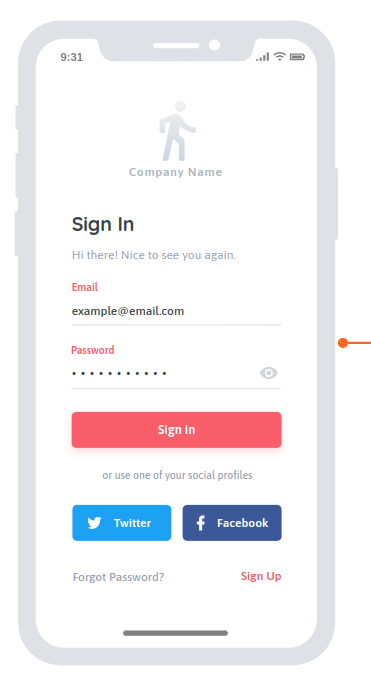
\includegraphics[width=20em]{./graphics/login_Mockup.png}
        \centering
        \caption{Mock up Login}
        \label{fig:loginMockup}
    \end{figure}

    \begin{figure}[htbp]
        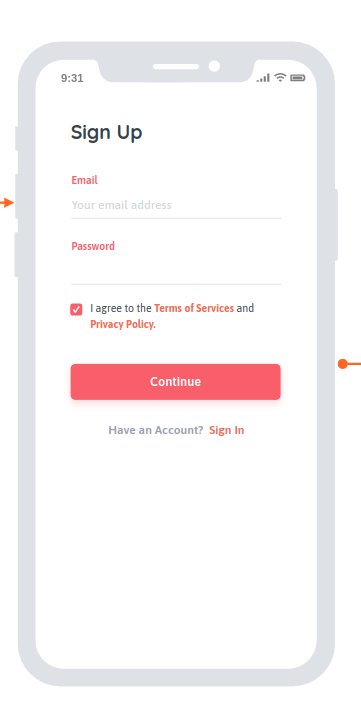
\includegraphics[width=20em]{./graphics/register_Mockup.png}
        \centering
        \caption{Mock up Register}
        \label{fig:registerMockup}
    \end{figure}
    
    \begin{figure}[htbp]
        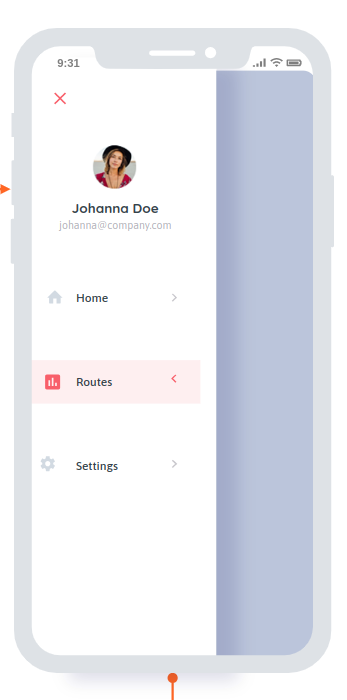
\includegraphics[width=20em]{./graphics/drawer_Mockup.png}
        \centering
        \caption{Mock up Drawer menu}
        \label{fig:DrawerMockup}
    \end{figure}

    \begin{figure}[htbp]
        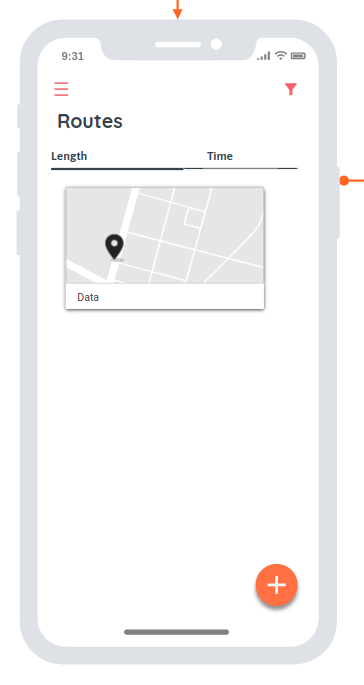
\includegraphics[width=20em]{./graphics/routeView_Mockup.png}
        \centering
        \caption{Mock up Route View}
        \label{fig:routeViewMockup}
    \end{figure}

    \begin{figure}[htbp]
        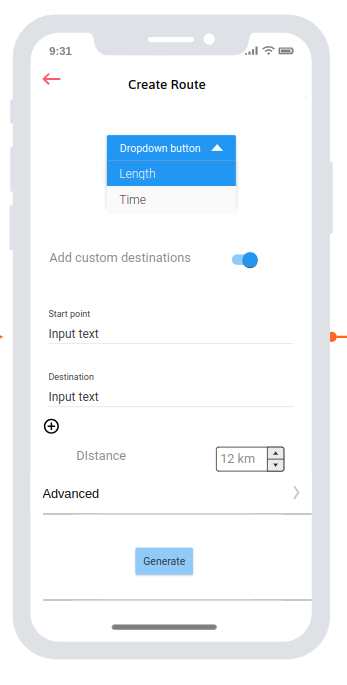
\includegraphics[width=20em]{./graphics/createRoute_Mockup.png}
        \centering
        \caption{Mock up Route Create}
        \label{fig:createRouteMockup}
    \end{figure}

    \begin{figure}[htbp]
        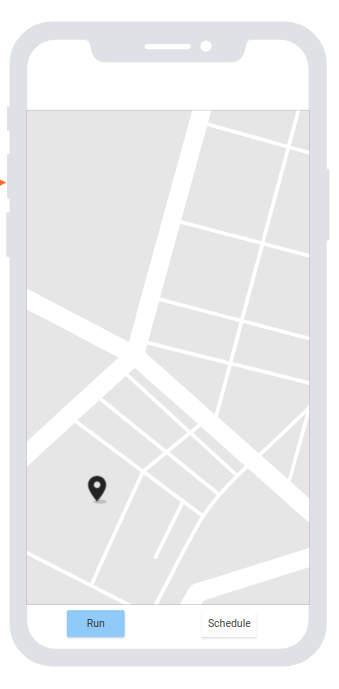
\includegraphics[width=20em]{./graphics/route_Mockup.png}
        \centering
        \caption{Mock up Route}
        \label{fig:routeMockup}
    \end{figure}

    \pagebreak

    \section{Proof of Concept}

    Na het ontwerp volgt de fase van ontwikkeling en implementatie. Hier wordt een Proof of Concept ontwikkeld, 
    bestaande uit zowel een online backend als een mobiele applicatie.

    De code is beschikbaar op Github. De frontend \url{https://github.com/LaurensDM/RunnerApp}.
    De backend \url{https://github.com/LaurensDM/RunnerApp-API}

    \subsection{Frontend}

    react-native-paper en react-native-navigation worden gebruikt voor styling en navigatie. 
    De applicatie is opgedeeld in verschillende componenten, 
    zoals HomeScreen, RouteScreen, SettingsScreen, SavedRoutesScreen, RouteCreateScreen en RouteDetailsScreen. 
    De navigatie tussen de verschillende schermen gebeurt via een drawer menu. 
    De applicatie maakt gebruik van Auth0 voor authenticatie en autorisatie. 
    De gebruiker kan inloggen met zijn e-mail en wachtwoord en wordt doorgestuurd naar het HomeScreen. 
    Gegevens worden opgeslagen in de lokale opslag van de mobiele applicatie via AsyncStorage 
    en gesynchroniseerd met de backend wanneer er een internetverbinding beschikbaar is.

    Om een route te genereren is een internetverbinding nodig, 
    maar een gebruiker kan een bestaande route terug ophalen en bekijken zonder internetverbinding.
    
    Hier is een overzicht van de verschillende schermen van de applicatie.
    
    Eerst wordt de gebruiker gevraagd om in te loggen. Hierbij wordt de gebruiker doorverwezen naar een browser waar Auth0 de authenticatie regelt.

    \begin{figure}[htbp]
        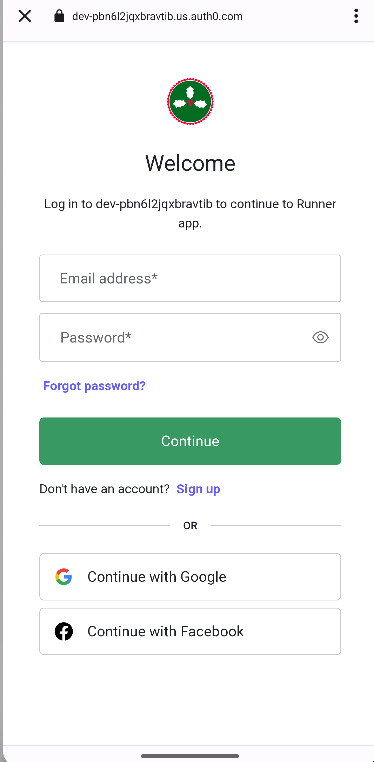
\includegraphics[width=20em]{./graphics/login.png}
        \centering
        \caption{Login}
        \label{fig:login}
    \end{figure}

    Vervolgens komt de gebruiker op het HomeScreen terecht. Voor de Proof of Concept staat hiet niet veel, 
    maar in de toekomst kan hier data van de gebruiker getoond worden.

    \begin{figure}[htbp]
        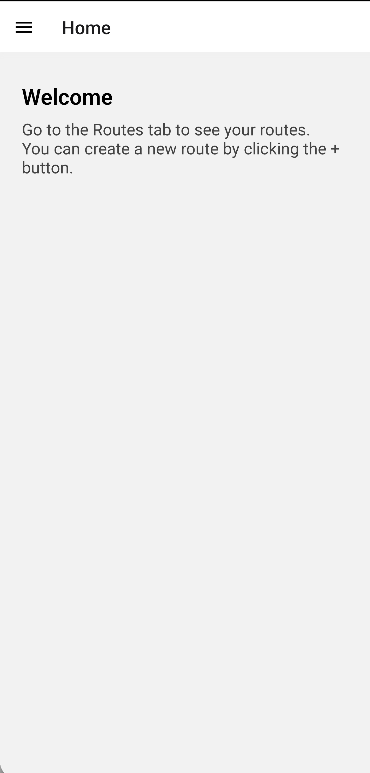
\includegraphics[width=20em]{./graphics/home.png}
        \centering
        \caption{Home}
        \label{fig:home}
    \end{figure}

    Via het drawer menu kan de gebruiker navigeren naar de verschillende schermen van de applicatie.

    \begin{figure}[htbp]
        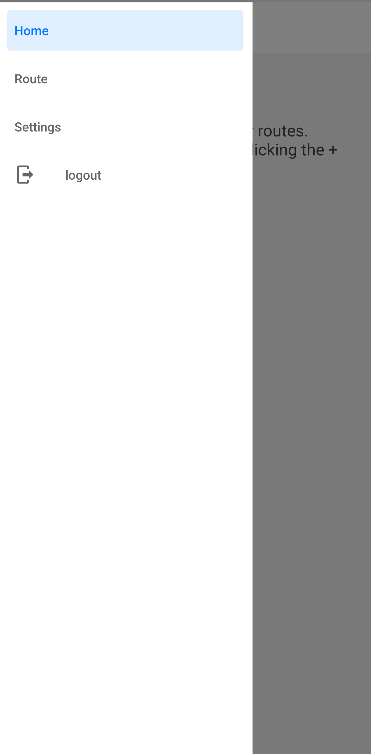
\includegraphics[width=20em]{./graphics/drawer.png}
        \centering
        \caption{Drawer}
        \label{fig:drawer}
    \end{figure}

    Op het Route scherm kan de gebruiker de opgeslagen routes bekijken en beheren.

    \subsection{Backend}
    
    De backend is ontwikkeld met behulp van Node.js en Express.js en communiceert met de frontend via een RESTful API. 
    Auth0 wordt gebruikt voor authenticatie en autorisatie. De gegevens worden opgeslagen in een MySQL database. 
    De backend communiceert verder met de Overpass API, Google Maps API en OpenWeatherMap API voor het genereren van looproutes en het opvragen van weersverwachtingen.
    
    Hier is een overzicht van de verschillende endpoints van de API.
    
    Het genereren van een route gebeurt in verschillende stappen. 
    De API krijgt eerst de nodige data binnen van de frontend, zoals de locatie van de gebruiker, de gewenste afstand of tijd van de route en verdere geavanceerde opties. 
    De API valideert eerst of alle nodige parameters aanwezig zijn met behulp van express-validator. 
    Vervolgens wordt een functie aangeroepen die de Overpass API aanspreekt om waypoints te genereren op basis van de gegeven parameters. 
    Functies die de Overpass API en Google Maps API aanspreken zijn gedefinieerd in een helpers folder, zodat er makkelijk integraties met andere platformen kunnen worden toegevoegd. 
    Met de waypoints wordt een for-loop gestart die de afstand tussen de waypoints berekent. Ook wordt hier de hoogte van de verschillende waypoints berekent en worden waypoints gefiltert 
    op basis van de gewenste hoogte die de gebruiker heeft gespecifieerd.
    Als de afstand tussen de waypoints groter is dan de gewenste afstand van de route,
    wordt de loop beëindigd zonder dat alle waypoints zijn inbegrepen. 
    In het geval dat er geen waypoints zijn teruggevonden, wordt een waypoint gegenereerd op basis van de locatie van de gebruiker, die zich dan op een aantal kilometers van de startlocatie bevindt. 
    De route wordt opgeslagen in de database en teruggegeven aan de frontend.

    \pagebreak

\begin{lstlisting}
    async function generateRunningRoute({ startPoint, endPoint, waypoints, distance, advancedOptions }: RouteProps) {

    const generatedWaypoints = await getGeneratedWaypoints(distance!, startPoint, advancedOptions.poiTypes, advancedOptions.surfaceType);

    const allWaypoints = [startPoint, ...waypoints, ...generatedWaypoints, endPoint];
    const runningRouteWaypoints: Waypoint[] = [];

    let accumulatedDistance = 0;

    for (let i = 0; i < allWaypoints.length - 1; i++) {
        const waypoint1 = allWaypoints[i];
        const waypoint2 = allWaypoints[i + 1];
        const distance = calculateDistance(waypoint1, waypoint2);
        accumulatedDistance += distance;
        if (accumulatedDistance <= distance * 1000) { // Convert km to meters
            runningRouteWaypoints.push(waypoint1);
        } else {
            break;
        }
    }

    // Generate route using Google Maps Directions API
    try {
        const response = await generateGoogleRoute(startPoint, endPoint, runningRouteWaypoints);
        return response.data;
    } catch (error) {        
        console.error('Error fetching route:', error.message);
        return null;
    }
    }
\end{lstlisting}

    